% !TeX root = er.tex

\chapter{Capteurs}\label{ch.sensors}

Un robot ne peut pas se déplacer sur une distance donnée dans une direction donnée simplement en réglant la puissance relative des moteurs des deux roues et leur durée d'action. Supposons que nous voulions que le robot se déplace en ligne droite. Si nous réglons la puissance des deux moteurs au même niveau, même de petites différences dans les caractéristiques des moteurs et des roues feront que le robot tournera légèrement sur le côté. Les inégalités de la surface sur laquelle le robot se déplace font également tourner les roues à des vitesses différentes. L'augmentation ou la diminution de la friction entre les roues et la surface peut affecter la distance parcourue en un laps de temps donné. Par conséquent, si nous voulons que le robot se déplace vers un mur situé à 1 m et s'arrête 20 cm devant, le robot doit \emph{détecter} l'existence du mur et s'arrêter lorsqu'il \emph{détecte} que le mur est à 20 cm.

Un \emph{capteur} est un composant qui mesure certains aspects de l'environnement. L'ordinateur du robot utilise ces mesures pour contrôler les actions du robot. L'un des capteurs les plus importants en robotique est le capteur de distance qui mesure la distance entre le robot et un objet. En utilisant plusieurs capteurs de distance ou en faisant tourner le capteur, il est possible de mesurer l'angle de l'objet par rapport à l'avant du robot. Les capteurs de distance peu coûteux utilisant la lumière infrarouge ou les ultrasons sont invariablement utilisés dans les robots éducatifs ; les robots industriels utilisent fréquemment des capteurs laser coûteux car ils sont très précis.

Le son et la lumière sont également utilisés pour les \emph{communications} entre deux robots, comme décrit dans le Chap.~\ref{ch.swarm}.

Une connaissance plus approfondie de l'environnement peut être obtenue en analysant les images prises par une caméra. Bien que les caméras soient très petites et peu coûteuses (tous les smartphones en possèdent une), la quantité de données contenues dans une image est très importante et les algorithmes de traitement d'image nécessitent d'importantes ressources informatiques. C'est pourquoi les caméras sont principalement utilisées dans des applications complexes comme les voitures à conduite autonome.

La section~\ref{s.classify} présente la terminologie des capteurs. La section~\ref{s.distance-sensors} présente les capteurs de distance, les capteurs les plus souvent utilisés par les robots éducatifs. Elle est suivie de la Sec.~\ref{s.cameras} sur les caméras, puis d'une courte section sur les autres capteurs utilisés par les robots (Sec.~\ref{s.other-sensors}). La section ~\ref{s.range} définit les caractéristiques des capteurs : portée, résolution, précision, exactitude. Le chapitre se termine par une discussion sur la non-linéarité des capteurs (Sec.~\ref{s.nonlinearity}).


\section{Classification des capteurs}\label{s.classify}

Les capteurs sont classés comme \emph{proprioceptif}\index{capteur!proprioceptif} ou \emph{extéroceptif}\index{capteur!exteroceptif}, et les capteurs extéroceptifs sont en outre classés comme \emph{actif} ou \emph{passif} (Fig.~\ref{fig.sensor-classification}). Un capteur proprioceptif mesure un élément interne au robot lui-même. L'exemple le plus connu est le compteur de vitesse d'une voiture qui mesure la vitesse de la voiture en comptant les rotations des roues (Sec.~\ref{s.wheel}). Un capteur extéroceptif mesure quelque chose d'extérieur au robot, comme la distance à un objet. Un capteur actif affecte l'environnement généralement en émettant de l'énergie : un télémètre sonar sur un sous-marin émet des ondes sonores et utilise le son réfléchi pour déterminer la distance. Un capteur passif n'affecte pas l'environnement : un appareil photo enregistre simplement la lumière réfléchie par un objet. Les robots utilisent invariablement certains capteurs extéroceptifs pour corriger les erreurs qui pourraient survenir avec les capteurs proprioceptifs ou pour prendre en compte les changements de l'environnement.

\begin{figure}
\begin{center}
\begin{tikzpicture}[node distance = 4mm and 1cm]
\node (sensor) { \textsf{capteur} };
\node (ex) [above right=of sensor] { \textsf{extéroceptif} };
\node (pro) [below right=of sensor] { \textsf{proprioceptif} };
\node (active) [above right=of ex] { \textsf{actif} };
\node (passive) [below right=of ex] { \textsf{passif} };
\draw (sensor) -- (pro);
\draw (sensor) -- (ex);
\draw (ex) -- (active);
\draw (ex) -- (passive);
\end{tikzpicture}
\caption{Classification des capteurs}\label{fig.sensor-classification}
\end{center}
\end{figure}

\section{Capteurs de distance}\label{s.distance-sensors}
\index{capteur!distance}

Dans la plupart des applications, le robot doit mesurer la distance qui le sépare d'un objet à l'aide d'un \textit{capteur de distance}. Les capteurs de distance sont généralement \emph{actifs} : ils émettent un signal et reçoivent ensuite sa réflexion (le cas échéant) par un objet (Fig.~\ref{fig.measure-d}). Une façon de déterminer la distance consiste à mesurer le temps qui s'écoule entre l'émission d'un signal et sa réception :
\begin{equation}
s = \frac{1}{2}vt\,,\label{eq.reflected}
\end{equation}
où $s$ est la distance, $v$ est la vitesse du signal et $t$ est le temps écoulé entre l'envoi et la réception du signal. Le facteur de moitié tient compte du fait que le signal parcourt la distance deux fois : jusqu'à l'objet et ensuite réfléchi. Une autre façon de reconstruire la distance est d'utiliser la triangulation, comme expliqué dans la section ~ref{s.triangulating-sensors}.

\begin{figure}
\begin{center}
\begin{tikzpicture}
\draw[xshift=-1mm] pic { robot };
\foreach \x in {14, 18, 22, 26, 30, 34}
\draw[blue] (\x mm,-10mm) arc[start angle=-30, end angle=30, radius=20mm];
\draw[fill] (38mm,0) circle[radius=3pt];
\foreach \x in {16, 20, 24, 28, 32, 36}
\draw[thick,dashed,red] (\x mm,-10mm) arc[start angle=210, end angle=150, radius=20mm];
\end{tikzpicture}
\end{center}
\caption{Mesurer la distance en émettant une onde et en recevant sa réflexion}\label{fig.measure-d}
\end{figure}

Les capteurs de distance bon marché reposent sur un autre principe : comme l'intensité d'un signal diminue avec la distance, la mesure de l'intensité d'un signal réfléchi donne une indication de la distance entre le capteur et un objet. L'inconvénient de cette méthode est que l'intensité du signal reçu est influencée par des facteurs tels que la réflectivité de l'objet.


\subsection{Capteurs de distance à ultrasons}
\index{Capteur!ultrasonique}

Les ultrasons sont des sons dont la fréquence est supérieure à $20\:000$ hertz, c'est-à-dire supérieure à la fréquence la plus élevée pouvant être entendue par l'oreille humaine. Il existe deux environnements où le son est meilleur que la vision : la nuit et dans l'eau. Les chauves-souris utilisent les ultrasons pour s'orienter lorsqu'elles volent la nuit, car après le coucher du soleil, il y a peu de lumière naturelle pour localiser la nourriture. Les navires et les sous-marins utilisent les ultrasons pour détecter des objets, car le son se propage beaucoup mieux dans l'eau que dans l'air. Vérifiez-le vous-même en vous baignant dans un lac boueux ou dans l'océan : à quelle distance pouvez-vous voir un ami ? Maintenant, demande-lui de produire un son en frappant deux objets l'un contre l'autre ou en tapant dans ses mains. A quelle distance pouvez-vous entendre ce son ? 

La vitesse du son dans l'air est d'environ $340$ m/s ou $34\:000$ cm/s. Si un objet se trouve à une distance de $34$ cm d'un robot, il ressort de l'équation~\ref{eq.reflected} qu'un signal ultrasonore se déplacera vers l'objet et sera réfléchi :

Un circuit électronique peut facilement mesurer des périodes de temps en millisecondes.

L'avantage des capteurs à ultrasons est qu'ils ne sont pas sensibles aux changements de couleur ou de réflectivité des objets, ni à l'intensité lumineuse de l'environnement. Ils sont toutefois sensibles à la texture : le tissu absorbe une partie du son, tandis que le bois ou le métal le réfléchit presque entièrement. C'est pourquoi les rideaux, les tapis et les dalles de plafond souples sont utilisés pour rendre les pièces plus confortables.

Les capteurs à ultrasons sont relativement bon marché et peuvent fonctionner dans des environnements extérieurs. Ils sont utilisés dans les voitures pour détecter de courtes distances, par exemple pour faciliter le stationnement. Leur principal inconvénient est que la mesure de la distance est plutôt lente, car la vitesse du son est bien inférieure à celle de la lumière. Un autre inconvénient est qu'ils ne peuvent pas être focalisés afin de mesurer la distance à un objet spécifique.

\subsection{Capteurs de proximité à infrarouge}
\index{capteur!infrarouge}\index{capteur!de proximité}

\emph{La lumière infrarouge} est une lumière dont la longueur d'onde est supérieure à celle de la lumière rouge, qui est la lumière de plus grande longueur d'onde que nos yeux peuvent voir. L'œil peut voir la lumière dont la longueur d'onde est comprise entre $390$ et $700$ nanomètres (un nanomètre est un millionième de millimètre). La lumière infrarouge a des longueurs d'onde comprises entre $700$ et $1000$ nanomètres. Elle est invisible pour l'œil humain et est donc utilisée dans la télécommande des téléviseurs et autres appareils électroniques.

Les capteurs de proximité sont des dispositifs simples qui utilisent la lumière pour détecter la présence d'un objet en mesurant l'intensité de la lumière réfléchie. L'intensité de la lumière diminue avec le carré de la distance de la source et cette relation peut être utilisée pour mesurer la distance approximative de l'objet. La mesure de la distance n'est pas très précise car l'intensité réfléchie dépend également de la réflectivité de l'objet. Un objet noir réfléchit moins de lumière qu'un objet blanc placé à la même distance. Un capteur de proximité ne peut donc pas faire la distinction entre un objet noir proche et un objet blanc placé un peu plus loin. C'est la raison pour laquelle ces capteurs sont appelés des capteurs de proximité et non des capteurs de distance. La plupart des robots éducatifs utilisent des capteurs de proximité car ils sont beaucoup moins chers que les capteurs de distance.

\subsection{Détecteurs de distance optique}\label{s.distance optique}
\index{capteur!optique}

La distance peut être calculée à partir de la mesure du temps écoulé entre l'envoi d'un signal lumineux et sa réception. La lumière peut être de la lumière ordinaire ou de la lumière provenant d'un laser. La lumière produite par un laser est \emph{cohérente} (voir ci-dessous).  Le plus souvent, les lasers utilisés pour mesurer la distance utilisent la lumière infrarouge, bien que la lumière visible puisse également être utilisée. Les lasers présentent plusieurs avantages par rapport aux autres sources de lumière. Premièrement, les lasers sont plus puissants et peuvent détecter et mesurer la distance d'objets lointains. Deuxièmement, un faisceau laser est hautement focalisé, ce qui permet de mesurer précisément l'angle par rapport à l'objet (Fig.~\ref{fig.beam}).

\begin{figure}
\begin{center}
\begin{tikzpicture}
\draw pic { robot };
\draw[fill] (20:5) circle[radius=3pt];
\draw[blue] (0,0) -- (17:5) arc[start angle=17, end angle=23, radius=5cm] -- cycle;
\draw[dashed,red] (0,0) -- (10:5) arc[start angle=10, end angle=30, radius=5cm] -- cycle;
\end{tikzpicture}
\end{center}
\caption{Largeur du faisceau de lumière laser (solide) et de lumière non-cohérente (pointillé)}\label{fig.beam}
\end{figure}

\begin{quote}
\begin{center}
\textbf{Lumière cohérente}
\end{center}
Trois types de lumière sont représentés sur la Fig.~\ref{fig.coherent}. La lumière du soleil ou d'une ampoule est appelée \emph{lumière blanche} car elle est composée de lumière de plusieurs couleurs (fréquences) différentes, émise à différents moments (phases) et émise dans différentes directions. Les diodes électroluminescentes (DEL) émettent une lumière monochromatique (lumière d'une seule couleur), mais elle n'est pas cohérente car ses phases sont différentes et elle est émise dans des directions différentes. Les lasers émettent une lumière cohérente : toutes les ondes ont la même fréquence et la même phase (chaque onde débute au même moment). Toute l'énergie d'une lumière est concentrée dans un faisceau étroit et la distance peut être calculée en mesurant le temps de parcours et la différence de phase de la lumière réfléchie.
\end{quote}

\begin{figure}
\begin{center}
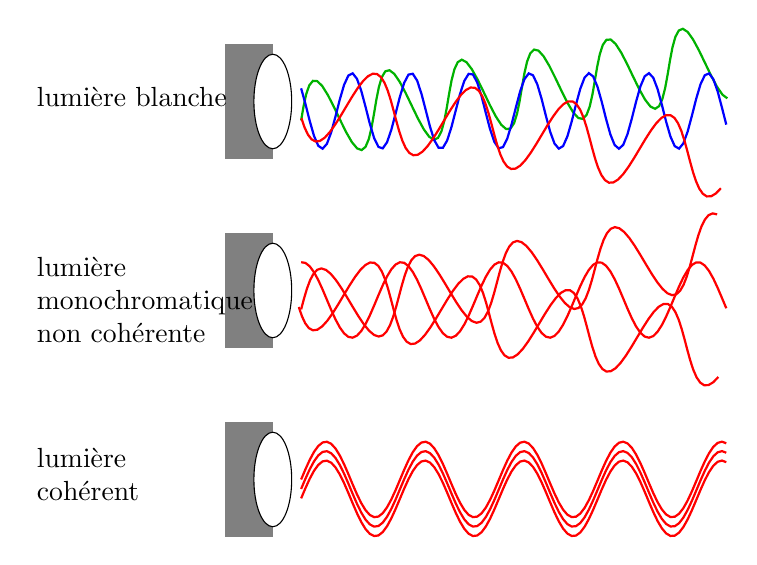
\begin{tikzpicture}[scale=.6,domain=0:9,align=left]
\draw[fill,gray] (-16mm,-8mm) rectangle +(10mm,24mm);
\draw[fill=white] (-6mm,4mm) circle[x radius=4mm, y radius=10mm];
\node[anchor=west] at (-5.8,5mm) {\p{lumière blanche}};
\draw[samples=100,green!70!black,thick,rotate=8] plot (\x,{.8*sin(4*\x r)});
\draw[samples=100,blue,thick,yshift=2mm] plot (\x,{.8*sin(5*(\x+.5) r)});
\draw[samples=100,red,thick,rotate=-8,yshift=4mm] plot (\x,{.8*sin(3*(\x+1.2) r)});
\begin{scope}[yshift=-4cm]
\draw[fill,gray] (-16mm,-8mm) rectangle +(10mm,24mm);
\draw[fill=white] (-6mm,4mm) circle[x radius=4mm, y radius=10mm];
\node[anchor=west] at (-5.8,2mm) {\p{lumière}\\\p{monochromatique}\\\p{non cohérente}};
\draw[samples=100,red,thick,rotate=8] plot (\x,{.8*sin(3*\x r)});
\draw[samples=100,red,thick,yshift=2mm] plot (\x,{.8*sin(3*(\x+.5) r)});
\draw[samples=100,red,thick,yshift=4mm,rotate=-8] plot (\x,{.8*sin(3*(\x+1.2) r)});
\end{scope}
\begin{scope}[yshift=-8cm]
\draw[fill,gray] (-16mm,-8mm) rectangle +(10mm,24mm);
\draw[fill=white] (-6mm,4mm) circle[x radius=4mm, y radius=10mm];
\node[anchor=west] at (-5.8,5mm) {\p{lumière}\\\p{cohérent}};
\draw[samples=100,red,thick] plot (\x,{.8*sin(3*\x r)});
\draw[samples=100,red,thick,yshift=2mm] plot (\x,{.8*sin(3*\x r)});
\draw[samples=100,red,thick,yshift=4mm] plot (\x,{.8*sin(3*\x r)});
\end{scope}
\end{tikzpicture}
\end{center}
\caption{Lumière blanche, monochromatique et cohérente}\label{fig.coherent}
\end{figure}

Supposons qu'une impulsion lumineuse soit transmise par le robot, réfléchie par un objet et reçue par un capteur sur le robot. La vitesse de la lumière dans l'air est d'environ $300\:000\:000$ m/s, soit $3\times 10^8$ m/s ou $3\times 10^{10}$ cm/s en notation scientifique. Si un signal lumineux est dirigé vers un objet situé à $30$ cm du robot, le temps d'émission et de réception du signal est (Fig.~\ref{fig.ir}):\index{temps écoulé du capteur}
\[
\frac{2\cdot 30}{3\times 10^{10}} = \frac{2}{10^9} = 2\times 10^{-9}\ \textrm{secondes} = 0,002\ \textrm{microsecondes}.
\]
C'est un laps de temps très court mais qui peut être mesuré par des circuits électroniques.

\begin{figure}
\includegraphics[width=.6\textwidth]{time-of-flight}
\caption{Un capteur de distance à temps de vol (noir) monté sur un circuit imprimé de 1,6 mm d'épaisseur (vert).}\label{fig.ir}
\end{figure}

Le deuxième principe de mesure de distance par un faisceau lumineux est la triangulation. Dans ce cas, l'émetteur et le récepteur sont placés à des endroits différents. Le récepteur détecte le faisceau réfléchi à une position qui est fonction de la distance de l'objet par rapport au capteur.

\subsection{Capteurs de triangulation}\label{s.triangulating-sensors}

Avant d'expliquer le fonctionnement d'un \emph{capteur de triangulation}\index{capteur!triangulation}, nous devons comprendre comment la réflexion de la lumière dépend de l'objet qu'elle rencontre. Lorsqu'un faisceau étroit de lumière, comme la lumière cohérente d'un laser, frappe une surface brillante comme un miroir, les rayons lumineux rebondissent en un faisceau étroit. L'angle de réflexion par rapport à la surface de l'objet est le même que l'angle d'incidence. C'est ce qu'on appelle la réflexion spéculaire (Fig.~\ref{fig.reflect-left}). Lorsque la surface est rugueuse, la réflexion est \emph{diffuse} (Fig.~\ref{fig.reflect-right}) dans toutes les directions car même les zones très proches de la surface ont des angles légèrement différents. La plupart des éléments présents dans un environnement, comme les personnes et les murs, ont une réflexion diffuse. Pour détecter la lumière laser réfléchie, il n'est donc pas nécessaire de placer le détecteur à un angle précis par rapport à l'émetteur.

\begin{figure}
\begin{minipage}{.45\textwidth}
\begin{tikzpicture}
\draw(5,0) arc[start angle=270, end angle=90, radius=8mm];
\begin{scope}[rotate=-15,xshift=-6mm,yshift=10mm]
\node[draw,rectangle,anchor=west,minimum height=5mm,minimum width=12mm,transform shape] (laser) at (0,8mm) {\p{Laser}};
\node[draw,rectangle,node distance=-.4pt,minimum height=2mm,minimum width=4mm,transform shape] (tip) [right=of laser] {};
\end{scope}
\draw(tip.east) -- ++(-15:28.5mm) -- +(195:30mm);
\end{tikzpicture}
\caption{Réflexion spéculaire\label{fig.reflect-left}}
\end{minipage}
\hspace{\fill}
\begin{minipage}{.45\textwidth}
\begin{tikzpicture}
\draw(5,0) arc[start angle=270, end angle=90, radius=8mm];
\begin{scope}[rotate=-15,xshift=-6mm,yshift=10mm]
\node[draw,rectangle,anchor=west,minimum height=5mm,minimum width=12mm,transform shape] (laser) at (0,8mm) {\p{Laser}};
\node[draw,rectangle,node distance=-.4pt,minimum height=2mm,minimum width=4mm,transform shape] (tip) [right=of laser] {};
\end{scope}
\draw(tip.east) -- ++(-15:28.5mm) coordinate (reflect) -- +(195:10mm);
\foreach \angle in {120,135,150,180,210,225}
  \draw(reflect) -- +(\angle:10mm);
\end{tikzpicture}
\caption{Réflexion diffuse\label{fig.reflect-right}}
\end{minipage}
\end{figure}

Les figures~\ref{fig.triangulation-left}--\ref{fig.triangulation-right} montrent un capteur à triangulation simplifié détectant un objet avec deux mesures de distance. Le capteur est constitué d'un émetteur laser et, à une distance $d$, d'une lentille qui focalise la lumière reçue sur un réseau de capteurs placés à une distance $l$ derrière la lentille. En supposant que l'objet reflète la lumière de manière diffuse, une partie de la lumière sera collectée par la lentille et focalisée sur les capteurs. La distance $d$ le long du réseau de capteurs est inversement proportionnelle à la distance $s$ de l'objet par rapport à l'émetteur laser.

Les triangles $\triangle ll'd$ et $\triangle ss'd$ sont similaires, nous avons donc la formule :
\[
\frac{s}{d} = \frac{l}{d'}\,.
\]
Comme $l$ et $d$ sont fixés par construction, en mesurant $d'$ à partir de l'indice du capteur qui détecte la lumière focalisée, on peut calculer $s$, la distance de l'objet au capteur. Le capteur doit être calibré en mesurant la distance $s$ correspondant à chaque capteur dans la matrice, mais une fois qu'une table est stockée dans l'ordinateur, la distance $s$ peut être effectuée par une consultation de la table.

De nombreux paramètres de conception affectent les performances d'un capteur de distance à triangulation : la puissance du laser, les caractéristiques optiques de l'objectif, le nombre de capteurs dans la matrice et leur sensibilité. Outre le compromis habituel entre performance et coût, le principal compromis se situe entre la portée et la distance minimale à laquelle un objet peut être mesuré. Pour une distance très courte $s$, la taille de la matrice de détecteurs $d'$ devient très grande, ce qui impose une limite pratique à la distance minimale. La distance minimale peut être réduite en augmentant la distance entre l'émetteur laser et le réseau de détecteurs, mais cela réduit la portée. Un capteur à triangulation peut être caractérisé par la distance $s_{\textit{opt}}$ pour une performance optimale, la distance minimale et la portée autour de $s_{\textit{opt}}$ à laquelle les mesures peuvent être effectuées.

\begin{figure}
\begin{minipage}{.5\textwidth}
\begin{tikzpicture}[scale=.65]
\draw(0,0) rectangle +(3,4);
\node[draw,rectangle,anchor=west,minimum height=5mm,minimum width=12mm] (laser) at (10mm,32mm) {\p{Laser}};
\node[draw,rectangle,node distance=-.4pt,minimum height=2mm,minimum width=2.4mm] (tip) [right=of laser] {};
\draw(26mm,20mm) coordinate (lens) ellipse [x radius=2mm, y radius=4mm];
\draw(28mm,14mm) node {\p{Lentille}};
\foreach \y in {8mm,10mm,12mm,14mm,16mm,18mm,20mm,22mm}
  \draw(10mm,\y) circle[radius=1mm];
\draw(11mm,4mm) node {\p{Réseau de détecteurs}};
\node[draw,rectangle,fill,color=lightgray,minimum height=8mm,minimum width=2mm] (object) at (70mm,32mm) {};
\draw(66mm,22mm) node {\p{Objet}};
% Triangles
\draw[thick,blue] (tip.east) -- node[right,black] {$d$} (lens.center);
\draw[thick,green!60!black,densely dashed] (lens.center) -- node[above,black] {$l$} +(-16mm,0) coordinate (sensor);
\draw[blue,thick] (sensor) -- node[left,black] {$d'$} ($ (object.west) ! 1.373 ! (lens.center) $) coordinate (sensor1);
\draw[densely dashed,thick,green!60!black] (tip.east) -- node[above,black] {$s$} (object.west);
\draw[red,thick] (object.west) -- ($ (object.west) ! 1.373 ! (lens.center) $) coordinate (sensor1);
\fill(tip.east) circle[radius=.8pt];
\fill(lens.center) circle[radius=.8pt];
\fill(sensor) circle[radius=.8pt];
\fill(sensor1) circle[radius=.8pt];
\node at (48mm,24mm) {$s'$};
\node at (18mm,14mm) {$l'$};
\end{tikzpicture}
\caption{Triangulation d'un objet éloigné}\label{fig.triangulation-left}
\end{minipage}
\hspace{\fill}
\begin{minipage}{.45\textwidth}
\begin{tikzpicture}[scale=.7]
\draw(0,0) rectangle +(3,4);
\node[draw,rectangle,anchor=west,minimum height=5mm,minimum width=12mm] (laser) at (10mm,32mm) {\p{Laser}};
\node[draw,rectangle,node distance=-.4pt,minimum height=2mm,minimum width=2.4mm] (tip) [right=of laser] {};
\draw(26mm,20mm) coordinate (lens) ellipse [x radius=2mm, y radius=4mm];
\draw(28mm,14mm) node {\p{Lentille}};
\foreach \y in {8mm,10mm,12mm,14mm,16mm,18mm,20mm,22mm}
  \draw(10mm,\y) circle[radius=1mm];
\draw(11mm,4mm) node {\p{Réseau de détecteurs}};
\node[draw,rectangle,fill,color=lightgray,minimum height=8mm,minimum width=2mm] (object) at (50mm,32mm) {};
\draw(46.5mm,22mm) node {\p{Objet}};
% Triangles
\draw[thick,blue] (tip.east) -- node[right,black] {$d$} (lens.center);
\draw[thick,green!60!black,densely dashed] (lens.center) -- node[above,black] {$l$} +(-16mm,0) coordinate (sensor);
\draw[blue,thick] (sensor) -- node[left,black] {$d'$} ($ (object.west) ! 1.7 ! (lens.center) $) coordinate (sensor1);
\draw[densely dashed,thick,green!60!black] (tip.east) -- node[above,black] {$s$} (object.west);
\draw[red,thick] (object.west) -- ($ (object.west) ! 1.7 ! (lens.center) $) coordinate (sensor1);
\fill(tip.east) circle[radius=.8pt];
\fill(lens.center) circle[radius=.8pt];
\fill(sensor) circle[radius=.8pt];
\fill(sensor1) circle[radius=.8pt];
\node at (38mm,24mm) {$s'$};
\node at (18mm,14mm) {$l'$};
\end{tikzpicture}
\caption{Triangulation d'un objet proche}\label{fig.triangulation-right}
\end{minipage}
\end{figure}

\subsection{Scanner laser}
\index{capteur!laser}

Lorsque des capteurs à ultrasons ou des capteurs de proximité sont utilisés, il est possible de placer un petit nombre de capteurs autour du robot afin de détecter des objets situés à proximité du robot (Fig.~\ref{fig.separate-sensors}). Bien entendu, l'angle par rapport à l'objet ne peut être mesuré avec précision, mais au moins l'objet sera détecté et le robot pourra s'en approcher ou l'éviter.

\begin{figure}
\begin{minipage}{.45\textwidth}
\begin{tikzpicture}
\draw pic { robot };
\draw[fill,blue] (10mm,5mm) circle[radius=2pt];
\draw[thin,blue] (10mm,5mm) -- +(45:10mm);
\draw[thin,blue] (10mm,5mm) -- +(-15:10mm);
\draw[fill,blue] (10mm,-5mm) circle[radius=2pt];
\draw[thin,blue] (10mm,-5mm) -- +(15:10mm);
\draw[thin,blue] (10mm,-5mm) -- +(-45:10mm);
\draw[fill,blue] (11mm,0mm) circle[radius=2pt];
\draw[thin,blue] (11mm,0mm) -- +(30:10mm);
\draw[thin,blue] (11mm,0mm) -- +(-30:10mm);
\draw[fill,blue] (-2mm,5mm) circle[radius=2pt];
\draw[thin,blue] (-2mm,5mm) -- +(140:10mm);
\draw[thin,blue] (-2mm,5mm) -- +(200:10mm);
\draw[fill,blue] (-2mm,-5mm) circle[radius=2pt];
\draw[thin,blue] (-2mm,-5mm) -- +(160:10mm);
\draw[thin,blue] (-2mm,-5mm) -- +(220:10mm);
\end{tikzpicture}
\caption{Cinq capteurs séparés}\label{fig.separate-sensors}
\end{minipage}
\hspace{\fill}
\begin{minipage}{.45\textwidth}
\begin{tikzpicture}[->]
\draw pic { robot };
\draw[dashed] (0,0) -- (2,0);
\draw (0,0) -- (150:2);
\draw[dashed] (.4,0) arc [start angle=0, end angle=150, radius=.4];
\draw[fill,blue] (0,0) circle[radius=2pt];
\end{tikzpicture}
\caption{Un capteur rotatif}\label{fig.rotating-sensor}
\end{minipage}
\end{figure}

Avec un capteur laser, la largeur du faisceau est si faible qu'un grand nombre de lasers (coûteux) serait nécessaire pour détecter des objets à n'importe quel angle. Une meilleure conception consiste à monter un seul capteur laser sur un arbre rotatif pour former un \emph{scanner laser} (Fig.~\ref{fig.rotating-sensor}). Un capteur angulaire peut être utilisé pour déterminer l'angle auquel un objet est détecté. Alternativement, l'ordinateur peut mesurer la période de temps après le passage du capteur rotatif dans une direction fixe. Une rotation complète de $360^\circ{}$ permet à un scanner laser de générer un profil des objets dans l'environnement (Fig.~\ref{fig.laser-scanner}).

\begin{figure}
\begin{center}
\includegraphics[width=.7\textwidth]{map-scanner}
\end{center}
\caption{Carte de l'environnement obtenue par un scanner laser}\label{fig.laser-scanner}
\end{figure}

\begin{framed}
\act{Distance d'un capteur de distance}{range}

\begin{itemize}
\item Déterminez la portée maximale à laquelle les capteurs de proximité de votre robot peuvent détecter un objet. Existe-t-il également une portée minimale où les objets peuvent être détectés même s'ils sont placés en contact direct avec le capteur ? S'il existe une portée minimale, expliquez pourquoi des objets plus proches ne peuvent pas être détectés.
\item Votre logiciel peut vous permettre de mesurer les valeurs numériques renvoyées par le capteur. Si tel est le cas, ces valeurs sont-elles des distances ou des valeurs arbitraires qui doivent être converties en distance ? S'il s'agit de valeurs arbitraires, trouvez une formule de conversion ou construisez un tableau qui donne les distances pour différentes valeurs renvoyées par le capteur.
\item Un capteur qui n'utilise pas de lumière laser cohérente peut détecter un objet à sa gauche ou à sa droite, et pas seulement les objets qui se trouvent directement devant lui. Mesurez l'angle auquel il est possible de détecter des objets. Les objets peuvent-ils être détectés au même angle à gauche et à droite du centre du capteur ?
\item Combien de capteurs faudrait-il pour pouvoir détecter un objet placé n'importe où autour de votre robot ?

\end{itemize}
\end{framed}

\medskip

\begin{framed}
\act{Seuils}{threshold}

\begin{itemize}
\item Un robot mobile comme une voiture autonome ne s'arrête pas exactement devant un obstacle ; il laisse un espace supplémentaire par sécurité, peut-être $1$ m ou $50$ cm. Définissez un \emph{threshold}\index{threshold}, la distance minimale de sécurité par rapport à un objet, et programmez votre robot pour qu'il s'arrête à cette distance d'un objet.
\item Si votre logiciel ne vous permet pas de mesurer les valeurs numériques renvoyées par le capteur, il peut vous permettre d'effectuer une action lorsque la valeur renvoyée passe un ou plusieurs seuils (par exemple, lorsque l'objet est " proche ", " moyen ", " éloigné "). Mesurez les distances correspondant à ces seuils : placez un objet à proximité du capteur et éloignez-le lentement. Notez les distances auxquelles les seuils sont franchis.
\end{itemize}
\end{framed}

\begin{framed}
\act{Réflectivité}{reflectivity}

\begin{itemize}
\item Puisqu'un capteur de proximité infrarouge fonctionne en mesurant la lumière réfléchie par un objet, il est raisonnable de supposer que les valeurs mesurées dépendent de la caractéristique de l'objet. Répétez les expériences de l'activité~\ref{act.range} pour des objets de formes, de couleurs et de matériaux différents. Résumez vos conclusions.
\item Essayez d'étendre la portée à laquelle votre capteur peut détecter un objet : utilisez un objet avec une surface métallique polie, fixez un miroir sur l'objet ou collez sur l'objet du ruban réfléchissant utilisé par les joggeurs et les cyclistes.
\item Si votre robot dispose d'un capteur à ultrasons, réalisez ces expériences pour ce capteur et comparez différentes textures de la surface d'un objet.
\end{itemize}
\end{framed}


\begin{framed}
\act{Triangulation}{dist-triangulation}

\begin{itemize}
\item Utilisez un pointeur laser pour créer un faisceau vers un objet placé à environ 50 cm. Tamisez les lumières ou fermez les rideaux des fenêtres afin de pouvoir voir la réflexion du faisceau sur l'objet. Placez ensuite un appareil photo sur une table ou un trépied à environ 10 cm du laser et pointez-le sur l'objet ; prenez ensuite une photo. Éloignez l'objet et prenez une autre photo. Qu'observez-vous lorsque vous comparez les deux photos ?
\item Déplacez l'objet de plus en plus loin du laser et de l'appareil photo, et notez les distances et la position du point sur la photo par rapport au bord de l'image. Tracez les données. Expliquez vos observations. Qu'est-ce qui définit la distance minimale et maximale que ce capteur peut mesurer ?
\end{itemize}
\end{framed}

\section{Caméras}\label{s.cameras}
\index{caméra}

Les appareils photo numériques sont largement utilisés en robotique car ils peuvent fournir des informations beaucoup plus détaillées que la simple distance et l'angle d'un objet. Les appareils photo numériques utilisent un composant électronique appelé \emph{dispositif à couplage de charge}\index{dispositif à transfert de charge (CCD, « Charge Coupled Device »)} qui détecte les ondes lumineuses et renvoie une matrice des \emph{pixels}\index{pixel} (Fig.~\ref{fig.camera}).

\begin{figure}
\includegraphics[width=.6\textwidth]{camera-image2}
\caption{Une image capturée par une caméra omnidirectionnelle avec un champ de vision de 360 degrés.}\label{fig.camera}
\end{figure}

Les appareils photo numériques se caractérisent par le nombre de pixels capturés dans chaque image et par le contenu de ces pixels. Une petite caméra utilisée dans un robot éducatif contient $192$ rangées de $256$ pixels chacune, soit un total de $49 152$ pixels. Il s'agit d'une très petite image : les capteurs des appareils photo numériques des smartphones enregistrent des images de millions de pixels.

Un appareil photo peut renvoyer les valeurs de chaque pixel en noir et blanc ($1$ bit par pixel), en nuances de gris appelées niveaux de gris ($8$ bits par pixel) ou en couleur rouge-vert-bleu (RVB) ($3$ fois $8=24$ bits par pixel). La petite caméra de $256\times 192$ a donc besoin d'environ $50$ kilo-octets pour une seule image en niveaux de gris ou $150$ kilo-octets pour une image en couleurs. Étant donné qu'un robot mobile tel qu'une voiture à conduite autonome devra stocker plusieurs images par seconde (les films et la télévision affichent $24$ images par seconde), la mémoire nécessaire pour stocker et analyser les images peut devenir très grande.

Une caractéristique importante dans la conception d'une caméra pour  robot est le \emph{champ de vision} de son objectif. Étant donné la position de la caméra, quelle partie de la sphère entourant la caméra est capturée dans l'image ? Pour un capteur donné dans une caméra, un objectif avec un champ de vision étroit capture une petite zone avec une haute résolution et peu de distorsion, tandis qu'un objectif avec un champ de vision large capture une grande zone avec une résolution plus faible et plus de distorsion. La distorsion la plus extrême provient d'une \emph{caméra omnidirectionnelle} qui capture en pratiquement une seule image toute la sphère qui l'entoure. La figure~\ref{fig.camera} montre l'image d'une salle de conférence prise par une caméra omnidirectionnelle ; la position de la caméra est indiquée par le point noir au centre. Les caméras à large champ de vision sont utilisées dans les robots mobiles car l'image peut être analysée pour comprendre l'environnement. L'analyse de l'image est utilisée pour la navigation, pour détecter des objets dans l'environnement et pour interagir avec des personnes ou d'autres robots en utilisant des propriétés visuelles comme la couleur.

Le problème fondamental des caméras en robotique est que nous ne sommes pas intéressés par un ensemble de pixels "bruts", mais par l'identification des objets présents dans l'image. L'œil et le cerveau humains effectuent instantanément des tâches de reconnaissance : lorsque nous conduisons une voiture, nous identifions automatiquement les autres voitures, les piétons, les feux de circulation et les obstacles sur la route, et nous prenons les mesures appropriées. Le traitement d'images par un ordinateur nécessite des algorithmes sophistiqués et une puissance de traitement importante (Chap.~\ref{ch.image}). Pour cette raison, les robots équipés de caméras sont beaucoup plus complexes et coûteux que les robots éducatifs qui utilisent des capteurs de proximité.

\section{Autres capteurs}\label{s.other-sensors}

Un \emph{capteur tactile}\index{capteur!tactile} peut être considéré comme un capteur de distance simplifié qui ne mesure que deux valeurs : la distance à un objet nulle ou supérieure à zéro. Les capteurs tactiles sont fréquemment utilisés comme mécanismes de sécurité. Par exemple, un capteur tactile est monté sur la partie inférieure des petits chauffages d'appoint afin que le chauffage ne fonctionne que si le capteur tactile détecte le sol. Si le radiateur tombe, le capteur tactile détecte qu'il n'est plus en contact avec le sol et le chauffage s'arrête pour éviter un incendie. Un capteur tactile peut être utilisé sur un robot mobile pour appliquer un arrêt d'urgence si le robot s'approche trop près d'un mur.

Des boutons et des interrupteurs permettent à l'utilisateur d'interagir directement avec le robot.

Un \emph{microphone}\index{sensor!microphone} sur le robot lui permet de détecter le son. Le robot peut simplement détecter le son ou utiliser des algorithmes pour interpréter les commandes vocales.

Un \emph{accéléromètre}\index{sensor!accelerometer} mesure l'accélération. L'utilisation principale des accéléromètres est de mesurer la direction de la force gravitationnelle qui provoque une accélération d'environ $9,8$ m/sec$^{2}$ vers le centre de la terre. Avec trois accéléromètres montés perpendiculairement les uns aux autres (Fig.~\ref{fig.accel}), on peut mesurer l' \emph{assiette} du robot : les trois angles du robot, appelés \emph{tangage}, \emph{lacet} et \emph{roulis}. Les accéléromètres sont abordés plus en détail dans la Sec.~\ref{s.accelerometer} et une activité utilisant des accéléromètres est présentée dans la Sec.~\ref{s.detect-slope}.

\begin{figure}
\begin{center}
\begin{tikzpicture}[->]
\draw pic { robot };
\draw (0,0,0) -- (0,0,3);
\draw (.3,0,2.6) arc [start angle=0, end angle=270, radius=4mm];
\draw (0,0,0) -- (0,2,0);
\draw (-.3,1.8,0) arc [start angle=-180, end angle=90, radius=3mm];
\draw (0,0,0) -- (2,0,0);
\draw (2.3,0,0) arc [start angle=0, end angle=270, radius=3mm];
\path (0,-16mm) -- +(0,1mm);  % So arrow doesn't get chopped
\node at (1,2) {\textsf{tangage}};
\node at (3,0) {\textsf{roulis}};
\node at (-2,-1) {\textsf{lacet}};
\end{tikzpicture}
\caption{Accéléromètre trois axes}\label{fig.accel}
\end{center}
\end{figure}

\begin{framed}
\act{Mesure de l'assiette à l'aide d'accéléromètres}{accelerometers}

\begin{itemize}
\item Écrivez un programme qui affiche l'assiette de votre robot lorsque vous le prenez et le faites tourner autour des trois axes.

\item Implémentez un jeu de votre choix en utilisant le robot comme contrôleur.

\item Écrivez un programme qui fait avancer le robot et qui s'arrête si une pente est atteinte. Utilisez l'accéléromètre pour mesurer l'inclinaison.
\end{itemize}
\end{framed}

\section{Etendue de mesure, résolution, précision, exactitude}\label{s.range}

Lorsqu'une quantité physique est mesurée, la mesure peut être caractérisée par son étendue, sa résolution, sa précision et son exactitude, des concepts souvent confondus.

L'\emph{gamme}\index{gamme} est l'étendue de l'ensemble des valeurs qui peuvent être mesurées par un capteur. Un capteur de proximité infrarouge pourrait être capable de mesurer des distances comprises entre 1$ cm et 30$ cm. Comme les faisceaux laser concentrent beaucoup de puissance dans un faisceau étroit, ils ont une portée beaucoup plus grande. La portée requise par un capteur de distance pour un robot se déplaçant dans un bâtiment sera d'environ 10 m, tandis qu'un capteur de distance pour une voiture autonome doit mesurer des distances d'environ 100 m.

\emph{Resolution}\index{resolution} fait référence au plus petit changement qui peut être mesuré. Un capteur de distance peut indiquer des distances en centimètres ($1$ cm, $2$ cm, $3$ cm, $4$ cm, \ldots), tandis qu'un meilleur capteur indique des distances en centièmes de centimètres ($4,00$ cm, $4,01$ cm, $4,02$ cm, \ldots). Pour une voiture autonome, une résolution de l'ordre du centimètre devrait suffire : on ne garerait pas une voiture à $1$ cm d'une autre, sans parler de la garer à $0,1$ cm. Un robot chirurgical a besoin d'une résolution beaucoup plus élevée, car le moindre millimètre est critique lors d'une opération.

\emph{Précision}\index{precision} fait référence à la cohérence de la mesure. Si la même quantité est mesurée à plusieurs reprises, la même valeur est-elle retournée ? La précision est très importante car des mesures incohérentes conduiront à des décisions incohérentes. Supposons qu'un capteur d'une voiture autonome mesure les distances à $10$ cm près, mais que les mesures successives renvoient une large gamme de valeurs (disons, $250$ cm, $280$ cm, $210$ cm). Lorsqu'elle essaie de maintenir une distance fixe avec un véhicule qu'elle suit, la voiture accélère et ralentit sans raison valable, ce qui rend la conduite inconfortable et gaspille de l'énergie.

Très souvent, un capteur aura une haute résolution mais une faible précision ; dans ce cas, on ne peut pas se fier à la résolution. Par exemple, un capteur de distance peut renvoyer des valeurs en millimètres, mais si la précision n'est pas suffisamment élevée, par exemple $45$ mm, $43$ mm, $49$ mm, le capteur ne peut renvoyer des valeurs que dans le centimètre ou le demi-centimètre le plus proche.

\begin{framed}
\act{Précision et résolution}{precision}
\begin{itemize}
\item Quelle est la résolution des capteurs de distance de votre robot ?
\item Placez un objet à une distance fixe de votre robot et enregistrez à plusieurs reprises la distance mesurée. Quelle est la précision de la mesure ?
\item Mesurez la distance d'un objet dans différentes circonstances telles que des changements de température et de lumière. Allumez et éteignez le chauffage ou le climatiseur ; allumez et éteignez les lumières. Les mesures changent-elles ?
\end{itemize}
\end{framed}

L' \emph{exactitude}\index{accuracy} fait référence à la proximité d'une mesure par rapport à la quantité réelle mesurée. Si un capteur de distance affirme systématiquement que la distance est supérieure de $5$ cm à ce qu'elle est en réalité, le capteur n'est pas précis. En robotique, l'exactitude n'est pas aussi importante que la précision, car la mesure d'un capteur ne renvoie pas directement une quantité physique. Au lieu de cela, un calcul est effectué pour obtenir une quantité physique telle que la distance ou la vitesse à partir d'une valeur électronique mesurée. Si l'imprécision est constante, la valeur du capteur peut être calibrée pour obtenir la véritable quantité physique (Sect.~\ref{s.nonlinearity}). Un capteur de distance utilisant la lumière ou le son calcule la distance à partir du temps de vol d'un signal $s=vt/2$. Si l'on sait que le capteur renvoie systématiquement une valeur de $5$ cm trop grande, l'ordinateur peut simplement utiliser la formule $s=(vt/2) - 5$.

\begin{framed}
\act{Exactitude}{accuracy}
\begin{itemize}
\item Placez un objet à différentes distances du robot et mesurez les distances renvoyées par le capteur. Les résultats sont-ils précis ? Si non, pouvez-vous écrire une fonction qui transforme les mesures du capteur en distances ?
\end{itemize}
\end{framed}

\section{Non linéarité}\label{s.nonlinearity}
\index{nonlinearity}

Les capteurs renvoient des grandeurs électroniques telles que la tension qui sont proportionnelles à ce qui est mesuré. Les valeurs analogiques sont converties en valeurs numériques. Par exemple, un capteur de proximité peut renvoyer $8$ bits de données (valeurs comprises entre $0$ et $255$) qui représentent une gamme de distances, peut-être de $0$ à $50$ cm. Un capteur de $8$ bits ne peut même pas renvoyer des angles de l'ordre de $0^\circ$--$360^\circ$ avec une résolution d'un degré. L'ordinateur doit traduire les valeurs numériques en mesures d'une quantité physique. La découverte de la correspondance pour cette traduction est appelée \emph{calibration}\index{calibration}. Dans le meilleur des cas, la correspondance sera linéaire et facile à calculer. Dans le cas contraire, si la correspondance est non linéaire, il faut utiliser une table ou une fonction non linéaire. Les tables sont plus efficaces car la recherche d'une entrée est plus rapide que le calcul d'une fonction, mais elles nécessitent beaucoup de mémoire.

\subsection{Capteurs linéaires}
\index{Capteur!linéaire}

Si un capteur de distance horizontal est \emph{linéaire}, il existe une correspondance $x = a s + b$, où $x$ est la valeur renvoyée par le capteur, $s$ est la distance d'un objet par rapport au capteur et $a,b$ sont des constantes ($a$ est la pente et $b$ l'interception avec l'axe du capteur). Supposons que le capteur renvoie la valeur $100$ pour un objet à $2$ cm et la valeur $0$ pour un objet à $30$ cm (Fig.~ref{fig.linear}).

\begin{figure}
\begin{center}
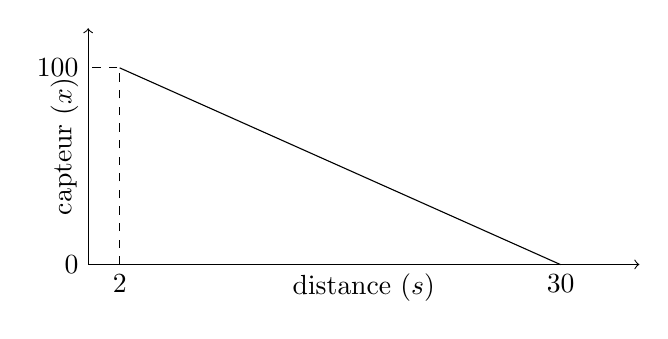
\begin{tikzpicture}
\draw[<->] (0,3) -- node[sloped,above,rotate=180] {\p{capteur ($x$)}} (0,0) node[left] {\p{0}} -- node[below] {\p{distance ($s$)}} (7,0);
\draw[dashed] (.4,0) node[below] {\p{2}} -- (.4,2.5) -- (0,2.5) node[left] {\p{100}};
\draw[domain=2:30] plot (\x/5,{(-3.57*\x+107)/40}) node[below] {\p{30}};
\end{tikzpicture}
\caption{Valeur renvoyée comme une fonction linéaire de la distance}\label{fig.linear}
\end{center}
\end{figure}

Calculons la pente et l'ordonnée à l'origine :
\[
\mathit{slope} = \frac{\Delta x}{\Delta s} = \frac{0-100}{30-2}=-3.57\,..
\]
Lorsque $s=30$, $x=0=-3,57\cdot 30+b$, donc $b=107$ et $x = -3,57 s + 107$. La résolution de $s$ donne une fonction que l'ordinateur du robot peut utiliser pour associer une valeur de capteur à la distance correspondante :
\[
s = \frac{107-x}{3,57}\,.
\]

\begin{framed}
\act{Linéarité}{linearity}
\begin{itemize}
\item Posez une règle sur votre table et placez soigneusement le robot de sorte que son
capteur avant soit placé à côté du repère $0$ de la règle. Placez un objet à côté de la marque de $1$ cm sur la règle. Notez la valeur renvoyée par le capteur. Répétez l'opération pour $2$ cm, $3$ cm, \ldots, jusqu'à ce que la valeur renvoyée devienne nulle.
\item Tracez un graphique de la valeur renvoyée en fonction de la distance. La réponse du capteur est-elle linéaire ? Si oui, calcule la pente et l'ordonnée à l'origine.
\item Répétez l'expérience avec des objets de formes et de matériaux différents. La linéarité du graphique dépend-elle des caractéristiques de l'objet ?
\end{itemize}
\end{framed}

\subsection{Capteurs non linéaires}

La figure~\ref{fig.nonlinear} montre un résultat possible des mesures de l'activité~\ref{act.linearity}. Les mesures sont représentées par des points et la fonction linéaire de la figure~{ref{fig.linear}. La fonction est raisonnablement linéaire au milieu de sa plage mais non linéaire en dehors de cette plage. Cela signifie qu'il est impossible d'utiliser une fonction linéaire des valeurs brutes du capteur pour obtenir la distance d'un objet par rapport au robot.

\begin{figure}
\begin{center}
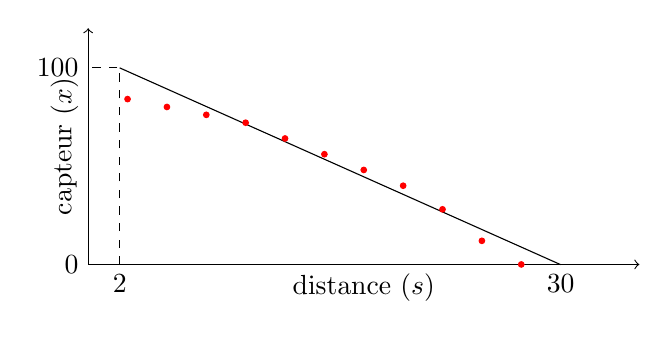
\begin{tikzpicture}
\draw[<->] (0,3) -- node[sloped,above,rotate=180] {\p{capteur ($x$)}} (0,0) node[left] {\p{0}} -- node[below] {\p{distance ($s$)}} (7,0);
\draw[dashed] (.4,0) node[below] {\p{2}} -- (.4,2.5) -- (0,2.5) node[left] {\p{100}};
\draw[domain=2:30] plot (\x/5,{(-3.57*\x+107)/40}) node[below] {\p{30}};
\foreach \x/\y in {0.5/2.5, 1/2.4, 1.5/2.3, 2/2.2, 2.5/2, 3/1.8, 3.5/1.6, 4/1.4, 4.5/1.1, 5/0.7, 5.5/0.4}
  \draw[fill,red,yshift=-4mm] (\x,\y) circle[radius=1pt];
\end{tikzpicture}
\caption{Valeurs expérimentales renvoyées en fonction de la distance}\label{fig.nonlinear}
\end{center}
\end{figure}

Nous pouvons construire un tableau pour faire correspondre les valeurs des capteurs aux distances. Le tableau~\ref{tab.nonlinear} est un tableau basé sur des mesures réelles avec un robot éducatif. Les mesures ont été effectuées tous les deux centimètres, de $2$ cm à $18$ cm ; à $20$ cm, le capteur ne détecte plus l'objet. La deuxième colonne indique la valeur du capteur pour chaque distance. La troisième colonne indique les valeurs $x_l$ qui seraient renvoyées par le capteur s'il était linéaire avec la fonction $x=-2s+48$. Nous voyons que les valeurs réelles renvoyées par le capteur ne s'écartent pas trop de la linéarité, il ne serait donc pas déraisonnable d'utiliser une fonction linéaire.

\begin{table}
\begin{displaymath}
\begin{array}{r@{\hspace{2em}}r@{\hspace{2em}}r}\hline
s \textrm{(cm)} & x & x_l\\\hline
18 &14 & 12\\
16 &18 & 16\\
 14&22 & 20\\
 12&26 & 24\\
 10&29 & 28\\
 8 &32 & 32\\
 6 &36 & 36\\
 4 &41 & 40\\
 2 &44 & 44\\
\end{array}
\end{displaymath}
\caption{Tableau de correspondance entre les valeurs des capteurs et les distances}\label{tab.nonlinear}
\end{table}


Évidemment, il serait préférable d'avoir une entrée de tableau pour chacune des valeurs possibles renvoyées par le capteur. Cependant, cela prendrait beaucoup de mémoire et pourrait s'avérer peu pratique si la plage des valeurs renvoyées par le capteur est beaucoup plus large, par exemple de $0$ à $4095$ ($12$ bits). Une solution consiste à prendre la valeur la plus proche, de sorte que si la valeur $27$ est renvoyée par le capteur dont le mappage est donné dans le Tableau~\ref{tab.nonlinear}, la distance sera de $12$.

Une meilleure solution consiste à utiliser l'interpolation\index{interpolation}. Si vous étudiez à nouveau le graphique de la Fig.~\ref{fig.nonlinear}, vous pouvez constater que les segments de la courbe sont à peu près linéaires, bien que leurs pentes changent en fonction de la courbe. Par conséquent, nous pouvons obtenir une bonne approximation de la distance correspondant à une valeur de capteur en prenant la distance relative sur une ligne droite entre deux points (Fig.~ref{fig.interpolation}). Étant donné les distances $s_1$ et $s_2$ correspondant aux valeurs de capteur $x_1$ et $x_2$, respectivement, pour une valeur $x_1<x<x_2$, sa distance $s$ :
\[
s = s_1 + \frac{s_2-s_1}{x_2-x_1}(x-x_1)\,.
\]

\begin{figure}
\begin{center}
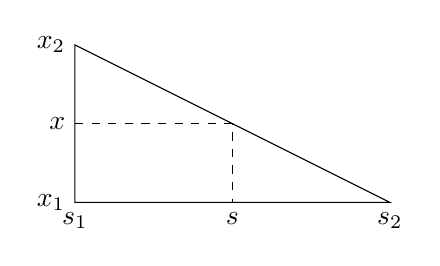
\begin{tikzpicture}
\draw (0,0) node[left] {$x_1$} -- (0,2) node[left] {$x_2$} -- (4,0) node[below] {$s_2$} -- cycle node[below] {$s_1$};
\draw[dashed] (0,1) node[left] {$x$} -| (2,1) -- (2,0) node[below] {$s$};
\end{tikzpicture}
\caption{Interpolation des valeurs du capteur}\label{fig.interpolation}
\end{center}
\end{figure}

\section{Résumé}

Lors de la conception d'un robot, le choix des capteurs est crucial. Le concepteur doit décider ce qui a besoin d'être mesuré : la distance, l'attitude, la vitesse, etc. Ensuite, le concepteur doit faire des compromis : une plus grande portée, une résolution plus fine, une plus grande précision et une meilleure exactitude ont un prix. Néanmoins, les principes algorithmiques sont les mêmes, que les capteurs soient de haute qualité ou non, de sorte que le compromis n'affecte pas la capacité d'apprentissage du robot.

Tout capteur connecté à l'ordinateur du robot va renvoyer des valeurs discrètes dans une plage fixe. L'ordinateur doit être en mesure d'associer ces valeurs de capteur à des quantités physiques dans le cadre d'un processus appelé étalonnage. Si le capteur est linéaire, l'étalonnage donne deux valeurs (pente et ordonnée à l'origine) qui déterminent une fonction linéaire. Si le capteur est non linéaire, une table ou une fonction non linéaire doit être utilisée.

 


\section{Pou aller plus loin}

Pour une vue d'ensemble des capteurs utilisés dans les robots mobiles, voir \cite[Section 4.1]{siegwart}. Le livre d'Everett \cite{everett} est entièrement consacré à ce sujet.
